Let us first give an example of a refinement of a poset and then introduce all notions we need formally.
\begin{example}
\label{ex:e1e2e3}
Let us consider the poset $(\{e_1,e_2,e_3,e_4\},\sqsubset)$ where $e_1\sqsubset_{O_1}e_2\sqsubset_{O_2}e_3$, $e_4\sqsubset_{O_4}e_3$ and $\labl(e_1)=r_1$, $\labl(e_2)=r_2$, $\labl(e_3)=r_3$, $\labl(e_4)=r_4$.

First we refine $r_2$ using the relation $r_1\redl{+}_{O_1} r_2$, (as we have seen in~\autoref{def:low_res}):
\[
\begin{tikzpicture} %[scale=0.8]
  \node (o1) at (0,-1) {\(O_1\)};
  \node (m1) at (0,1) {\(M_1\)};
  \node (n1) at (2,1) {\(N_1\)};
  \node (r1) at (-1,0) {\(R_1\)};
  \node (l1) at (-2.5,0) {\(L_1\)};
  \node (l2) at (1,0) {\(L_2\)};
  \node (r2) at (2.5,0) {\(R_2\)};
  \draw [->] (o1) -- (r1);
  \draw [->] (o1) -- (l2);
  \draw [->] (r1) -- (m1);
  \draw [->] (r2) -- (n1);
  \draw [->] (l2) -- (m1);
  \draw [vecArrow] (l1) -- (r1);
  \draw [vecArrow] (m1) -- (n1);
  \draw [vecArrow] (l2) -- (r2);
\end{tikzpicture}
\]
We apply a rewriting step to $M_1$ using rule $r_2$ to obtain $N_2$. We refine then $r_3$ using $N_2$ (this step is formally defined in~\autoref{def:seq_comb}):
\[
\begin{tikzpicture} %[scale=0.8]
  \node (o1) at (0,-1) {\(O_1\)};
  \node (m1) at (0,1) {\(M_1\)};
  \node (r1) at (-1,0) {\(R_1\)};
  \node (l1) at (-2.5,0) {\(L_1\)};
  \node (l2) at (1,0) {\(L_2\)};
  \node (r2) at (2.5,0) {\(R_2\)};
  \node (o2) at (3.5,-1) {\(O_2\)};
  \node (l3) at (4.5,0) {\(L_3\)};
  \node (r3) at (6,0) {\(R_3\)};
  \node (m2p) at (2.5,1) {\(N_1\)};
  \node (n) at (3.5,2) {\(M_2\)};
  \node (n2) at (5,2) {\(N_2\)};
  \draw [->] (o1) -- (r1);
  \draw [->] (o1) -- (l2);
  \draw [->] (r1) -- (m1);
  \draw [->] (l2) -- (m1);
  \draw [->] (o2) -- (r2);
  \draw [->] (o2) -- (l3);
  \draw [->] (l3) -- (n);
  \draw [->] (m2p) -- (n);
  \draw [->] (r2) -- (m2p);
  \draw [->] (r3) -- (n2);
  \draw [vecArrow] (l1) -- (r1);
  \draw [vecArrow] (l2) -- (r2);
  \draw [vecArrow] (l3) -- (r3);
  \draw [vecArrow] (m1) -- (m2p);
  \draw [vecArrow] (n) -- (n2);
\end{tikzpicture}
\]
Let us now integrate $e_4\sqsubset_{O_4} e_3$ in the sequence. Let $R_4\lemb M_3\remb L_3$ be the cospan obtained from $\labl(e_4)\redl{+}_O\labl(e_3)$.
We combine $M_2$ and $M_3$ using $L_3$ (concurrent combinator is formally introduced in~\autoref{def:conc_comb}):
\[
\begin{tikzpicture} %[scale=0.8]
  \node (l4) at (0.5,0) {\(L_4\)};
  \node (r4) at (2,0) {\(R_4\)};
  \node (o4) at (3,-1) {\(O_4\)};
  \node (m4) at (3,1) {\(M_3\)};
  \node (l3) at (4,0) {\(L_3\)};
  \node (r3) at (5.5,0) {\(R_3\)};
  \node (m2p) at (5,1) {\(M_2\)};
  \node (n) at (4,2) {\(M_4\)};
  \draw [->] (o4) -- (r4);
  \draw [->] (o4) -- (l3);
  \draw [->] (r4) -- (m4);
  \draw [->] (l3) -- (m4);
  \draw [->] (m4) -- (n);
  \draw [->] (m2p) -- (n);
  \draw [->] (l3) -- (m2p);
  \draw [vecArrow] (l4) -- (r4);
  \draw [vecArrow] (l3) -- (r3);
\end{tikzpicture}
\]
The refinement of our poset is then the following set of transitions:
\[
\begin{tikzpicture} %[scale=0.8]
  \node (o1) at (0,-1) {\(O_1\)};
  \node (m1) at (0,1) {\(M_1\)};
  \node (r1) at (-1,0) {\(R_1\)};
  \node (l1) at (-2.5,0) {\(L_1\)};
  \node (l2) at (1,0) {\(L_2\)};
  \node (r2) at (2.5,0) {\(R_2\)};
  \node (o2) at (3.5,-1) {\(O_2\)};
  \node (l3) at (4.5,0) {\(L_3\)};
  \node (r3) at (6,0) {\(R_3\)};
  \node (n1) at (2.5,1) {\(N_1\)};
  \node (m2) at (3.5,2) {\(M_2\)};
  \node (m4) at (3.5,3) {\(M_4\)};
  \node (n4) at (6,3) {\(N_4\)};
  \draw [->] (o1) -- (r1);
  \draw [->] (o1) -- (l2);
  \draw [->] (r1) -- (m1);
  \draw [->] (l2) -- (m1);
  \draw [->] (o2) -- (r2);
  \draw [->] (o2) -- (l3);
  \draw [->] (l3) -- (m2);
  \draw [->] (n1) -- (m2);
  \draw [->] (r2) -- (n1);
  \draw [->] (r3) -- (n4);
  \draw [vecArrow] (l1) -- (r1);
  \draw [vecArrow] (l2) -- (r2);
  \draw [vecArrow] (l3) -- (r3);
  \draw [vecArrow] (m1) -- (n1);
  \draw [->] (m2) -- (m4);
  \draw [vecArrow] (m4) -- (n4);
\end{tikzpicture}
\]

%% Lastly we have to propagate $M_4$ backwards to events $e_1$, $e_2$ and $e_4$.
%% \[
%% \begin{tikzpicture} %[scale=0.8]
%%   \node (o1) at (0,-1) {\(O_1\)};
%%   \node (m1) at (0,1) {\(M_1\)};
%%   \node (r1) at (-1,0) {\(R_1\)};
%%   \node (l1) at (-2.5,0) {\(L_1\)};
%%   \node (l2) at (1,0) {\(L_2\)};
%%   \node (r2) at (2.5,0) {\(R_2\)};
%%   \node (o2) at (3.5,-1) {\(O_2\)};
%%   \node (l3) at (4.5,0) {\(L_3\)};
%%   \node (r3) at (6,0) {\(R_3\)};
%%   \node (n1) at (2.5,1) {\(N_1\)};
%%   \node (m2) at (3.5,2) {\(M_2\)};
%%   \node (n2) at (6,2) {\(N_2\)};
%%   \node (m6) at (-2.5,3) {\(M_6\)};
%%   \node (m5) at (0,3) {\(M_5\)};
%%   \node (m4) at (3.5,3) {\(M_4\)};
%%   \node (n4) at (6,3) {\(N_4\)};
%%   \draw [->] (o1) -- (r1);
%%   \draw [->] (o1) -- (l2);
%%   \draw [->] (r1) -- (m1);
%%   \draw [->] (l2) -- (m1);
%%   \draw [->] (o2) -- (r2);
%%   \draw [->] (o2) -- (l3);
%%   \draw [->] (l3) -- (m2);
%%   \draw [->] (n1) -- (m2);
%%   \draw [->] (r2) -- (n1);
%%   \draw [->] (r3) -- (n2);
%%   \draw [vecArrow] (l1) -- (r1);
%%   \draw [vecArrow] (l2) -- (r2);
%%   \draw [vecArrow] (l3) -- (r3);
%%   \draw [vecArrow] (m1) -- (n1);
%%   \draw [vecArrow] (m2) -- (n2);
%%   \draw [->] (n2) -- (n4);
%%   \draw [->] (m2) -- (m4);
%%   \draw [->] (m1) -- (m5);
%%   \draw [->] (l1) -- (m6);
%%   \draw [vecArrow] (m4) -- (n4);
%%   \draw [vecArrow] (m4) -- (m5);
%%   \draw [vecArrow] (m5) -- (m6);
%% \end{tikzpicture}
%% \]
%% The refinement of our poset is then the set of transitions
%% \[
%% \begin{tikzpicture} %[scale=0.8]
%%   \node (m6) at (0,1) {\(M_6\)};
%%   \node (m5) at (1.5,1) {\(M_5\)};
%%   \node (m4) at (3,1) {\(M_4\)};
%%   \node (n4) at (4.5,1) {\(N_4\)};
%%   \node (m7) at (1.5,0) {\(M_7\)};
%%   \draw [vecArrow] (m4) -- (n4);
%%   \draw [vecArrow] (m5) -- (m4);
%%   \draw [vecArrow] (m6) -- (m5);
%%   \draw [vecArrow] (m7) -- (m4);
%% \end{tikzpicture}
%% \]
%% where $M_7$ is obtained by a rewriting of $M_4$ using rule $r_4$.
\end{example}

\begin{definition}[Refinement of a rule~\cite{information_carriers}]
  Let $r:L{\Rightarrow} R$ be a rule and let $m:L\emb M$ be a matching in a graph $M$. The production $M\overset{m,r}{\Rightarrow} N$ obtained by DPO rewriting of $M$ using the rule $r$ is called a \emph{refinement} of $r$.
\end{definition}

\begin{definition}[Refinement of a poset]
  \label{def:ref_poset}
  Given a poset $s=(E,<,\labl)$ of graph rewriting events, the \emph{refinement} of $s$, is a bijection $\imath$ between events $e\in E$ and transitions $M\overset{m,p}{\Rightarrow} M'$ such that
  \begin{itemize}
  \item the label of an event is rule in the transition: $\labl(e)=p$;
  \item for all $e_1,e_2\in E$, if $e_1<e_2$ and $\imath(e_1) = M_1\overset{m_1,p_1}{\Rightarrow} M_1'$, $\imath(e_2) =M_2\overset{m_2,p_2}{\Rightarrow} M_2'$ then $M_1'\emb M_2$.
  \end{itemize}
\end{definition}

%Before giving the construction of a refinement $(M_i\overset{m_i,p_i}{\Rightarrow} M_{i+1})_{e_i\in E}$ let us first introduce some combinators of contexts.

%% \begin{definition}[Propagate a context]
%%   \label{def:propagate}
%%   Given a sequence $M_1{\Rightarrow} M_2\cdots {\Rightarrow} M_n\cdots {\Rightarrow} M_{m}$ and a graph $M_{n}'$ with $M_n\emb M_{n}'$ define the \emph{propagation} of $M_{n}'$ as the sequence  $M_1'{\Rightarrow} M_2'\cdots {\Rightarrow} M_n'\cdots {\Rightarrow} M_{m}'$ where
%%   \begin{itemize}
%%   \item $M_i'$, for $i<n$, is obtained by the reverse of the production $M_i\Rightarrow M_{i+1}$ applied to the new contexts;
%%   \item $M_i'$, for $n<i\leq m$, is obtained by the production $M_i\Rightarrow M_{i+1}$ applied to the new contexts.
%%   \end{itemize}
%% \end{definition}

\begin{definition}[Sequential combinator]
\label{def:seq_comb}
  Let $M\Rightarrow N$ and $L\Rightarrow R$ be two productions such that there exists $N\remb O \lemb L$ a cospan.
  Define the sequential combinator as follows:
  \[
  (M\overset{m,p}{\Rightarrow}N)\oplus_O (L\Rightarrow R) = M'\overset{m',p'}{\Rightarrow}N'
  \]
  where $N\emb M' \remb L$ is the pushout of the cospan $N\remb O \lemb L$ and $N'$ is obtained by a DPO rewriting of $M'$ by the production $L\Rightarrow R$:
  \[
  \begin{tikzpicture} %[scale=0.8]
    \node (o) at (0,-1) {\(O\)};
    \node (mp) at (0,1) {\(M'\)};
    \node (m) at (-2.5,0) {\(M\)};
    \node (n) at (-1,0) {\(N\)};
    \node (l) at (1,0) {\(L\)};
    \node (r) at (2.5,0) {\(R\)};
    \node (np) at (2,1) {\(N'\)};
    \draw [->] (o) -- (n);
    \draw [->] (o) -- (l);
    \draw [->] (n) -- (mp);
    \draw [->] (l) -- (mp);
    \draw [->] (r) -- (np);
    \draw [vecArrow] (m) -- (n);
    \draw [vecArrow] (l) -- (r);
    \draw [vecArrow] (mp) -- (np);
  \end{tikzpicture}
  \]
  We denote $m'$ the morphism $L\to M'$ and $p'$ the production $L\Rightarrow R$.
\end{definition}

\begin{definition}[Wide pushout~\cite{wide}]
The wide pushout of a family of morphisms $(P\to M_i)_i$ consists of a graph $M$ and a family of morphisms $(M_i\to M)_i$ such that the diagram commutes
\[
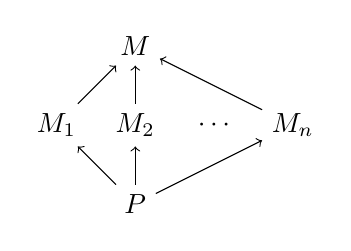
\begin{tikzpicture} %[scale=0.8]
  \node (o) at (0,-1) {\(P\)};
  \node (m1) at (-1,0) {\(M_1\)};
  \node (m2) at (0,0) {\(M_2\)};
  \node (text) at (1,0) {\(\cdots\)};
  \node (mn) at (2,0) {\(M_n\)};
  \node (m) at (0,1) {\(M\)};
  \draw [->] (o) --  (m1);
  \draw [->] (o) --  (m2);
  \draw [->] (o) --  (mn);
  \draw [->] (m1) --  (m);
  \draw [->] (m2) --  (m);
  \draw [->] (mn) --  (m);
\end{tikzpicture}
\]
for any other $M'$ and family of morphisms $(M_i\to M')_i$ there exists a unique morphism $M\to M'$ that commutes.

The wide pushout is equivalent to computing the pushout pairwise on $(P\to M_i)_i$.
\end{definition}

\begin{lemma}[Concurrent combinator]
  \label{def:conc_comb}
  Let $(M_i)_{0< i< n}$ be a family of graphs, let $(M'\emb M_i)_{0< i< n}$ be a family of injective morphisms and let $p:L\Rightarrow R$ be a production.
  Define the concurrent combinator as follows:
  \[
  \otimes_{L{\Rightarrow}R}(M_1, M_2,\cdots M_n) = M \overset{m,p}{\Rightarrow} N
  \]
  where $M$ is the wide pushout of the family of morphisms $(L\emb M_i)_i$.

  The morphisms $m_i$, obtained by the composition of $L\emb M_i$ and $M_i\emb M$ are equivalent. We denote $m$ one such morphism.

  The graph $N$ is obtained by a DPO rewriting of $M$ by the production $p$.
\end{lemma}
\begin{proof}
  First we prove that the morphisms $m_i$ obtained by the composition of $M'\emb M_i$  and $M_i\emb M$ are equivalent.
% which follows from the definition of the pushout.
  Secondly we show that the gluing conditions hold for the DPO rewriting of $p$ on $M$ iff they hold for the dpo rewriting of $p$ on all $M_i$. Both follow from $(M_i\to M)_i$ being the wide pushout of $(L\to M_i)_i$.
\end{proof}

\begin{definition}[Refinement propagation]
  \label{def:ref_propagator}
  Let $s=(E,\tleq,\labl)$ be a poset and let $(E,\sqsubset,\labl)\in \decor(s)$ be a decoration of $s$.
  We define a function, called the \emph{forward propagator}, by induction on $s$:
  \begin{align*}
    &\fp(e) = L\Rightarrow R&\text{ if }e\in\text{min}(s)\text{ and }\labl(e) = L\action R\\
    &\fp(e) = M\overset{m,p}{\Rightarrow} N&\text{ where }\forall e_i, e_i\sqsubset_{O_i}e,
    \fp(e_i)\oplus_{O_i}L\Rightarrow R= M_i\overset{m_i,p}{\Rightarrow} N_i\\
    &&\otimes_{\labl(e)}(M_1, M_2, \cdots M_n) = M \overset{m,p}{\Rightarrow} N
    \text{and }\labl(e) = p:L\action R\\
  \end{align*}
\end{definition}

\begin{lemma}
  $(E,\sqsubset,\labl,\fp)$ is a refinement of $(E,<,\labl)$.
\end{lemma}
\begin{proof}
  For the base case we have only to show that, for $\fp(e) = M\overset{m,p}{\Rightarrow} N$, $\labl(e)=p$. This follows from~\autoref{def:seq_comb} and~\autoref{def:conc_comb}.

  For the inductive case, let us consider an event $e$. As above, we have that if $\fp(e) = M\overset{m,p}{\Rightarrow} N$ then $\labl(e)=p$. If there exists $e'$, $e'\sqsubset_O e$ with $\fp(e')= M'\overset{m',p'}{\Rightarrow} N'$ then, from~\autoref{def:ref_propagator} and from~\autoref{def:seq_comb}, there exists $M''$ such that $M'\emb M''$. Moreover, from~\autoref{def:conc_comb}, $M''\emb M$.
\end{proof}

%% \begin{definition}[Refinement propagation]
%%   \label{def:ref_propagator}
%%   Let us define two functions the forward propagator $\fp$, and the backward propagator $\bp$, that map events in a poset $\{E,\sqsubset,\labl\}$ to transitions.
%% We proceed by induction on the transitive and reflexive closure of the cover relation $\sqsubset$ and start with the minimal events for the definition of $\fp$. For the definition of $\bp$ we proceed by induction on the transitive and reflexive closure of the reverse relation $\sqsubset^{-1}$ starting with the maximal events for $\bp$:
%% \begin{align*}
%%   \text{forward propagator}\\
%%   &\fp(e) = \labl(e)&\text{ if }e\in\text{min}(s)\\
%%   &\fp(e) = M\Rightarrow N&\text{ where }\forall e_i, e_i\sqsubset_{O_i}e, \fp(e_i)\oplus_{O_i}\labl(e) = M_i\Rightarrow N_i\\
%%   &&\otimes_{\labl(e)}(M_1, M_2, \cdots M_n) = M \Rightarrow N\\
%%   \\
%%   \text{backward propagator}\\
%%   &\bp(e) = \fp(e)&\text{ if }e\in\text{max}(s)\\
%%   &\bp(e) = M\Rightarrow N&\text{ where }\forall e_i, e\sqsubset_{O_i}e_i, \bp(e_i) = M_i\Rightarrow N_i\\
%%   &&\otimes_{\fp(e)^{-1}}(M_1, M_2, \cdots M_n) = M \Rightarrow N
%% \end{align*}
%% \end{definition}

%% \begin{definition}[Embeddings between transitions]
%%   A transition $M'\overset{m',p}\Rightarrow N'$ embeds into a transition $M\overset{m,p}\Rightarrow N$ if there exists a morphism $h:M'\to M$ such that the diagram commutes:
%%   \[
%%   \begin{tikzpicture} %[scale=0.8]
%%     \node (d) at (0,2.5) {\(D\)};
%%     \node (m) at (-2,2.5) {\(M\)};
%%     \node (n) at (2,2.5) {\(N\)};
%%     \node (m1) at (-2,1) {\(M'\)};
%%     \node (d1) at (0,1) {\(D'\)};
%%     \node (n1) at (2,1) {\(N'\)};
%%     \node (l) at (-2,-0.5) {\(L\)};
%%     \node (k) at (0,-0.5) {\(K\)};
%%     \node (r) at (2,-0.5) {\(R\)};
%%     \draw [left hook->] (l) -- node [right,midway] {$m'$} (m1);
%%     \draw [left hook->] (r) -- (n1);
%%     \draw [left hook->] (k) -- (d1);
%%     \draw [left hook->] (k) -- (l);
%%     \draw [left hook->] (k) -- (r);
%%     \draw [dotted, left hook->] (m1) -- (m);
%%     \draw [dotted, left hook->] (d1) -- (d);
%%     \draw [dotted, left hook->] (n1) -- (n);
%%     \draw [left hook->] (d1) -- (m1);
%%     \draw [left hook->] (d1) -- (n1);
%%     \draw [left hook->] (d) -- (m);
%%     \draw [left hook->] (d) -- (n);
%%     \draw [left hook->] (l) to [bend left] node [left,midway] {$m$} (m);
%%     \draw [left hook->] (k) to [bend right] (d);
%%     \draw [left hook->] (r) to [bend right] (n);
%%   \end{tikzpicture}
%%   \]
%% \end{definition}

%% \begin{lemma}
%%   \label{lem:subposet}
%%   Let $s'\subseteq s$ be a connected poset (i.e. directed either upwards or downwards). Then
%%   \[\forall e\in s', \bp_{s'}(e)\text{ embeds into }\bp_s(e),\]
%%   where $\bp_s(e)$ is the refinement of~\autoref{def:ref_propagator} applied to $s$.
%%   A \textbf{corollary} is that if two transitions are sequential dependent in $\bp_{s'}$ then they are sequential dependent in $\bp_{s}$.
%% \end{lemma}
%% \begin{proof}
%%   \begin{mdframed}[backgroundcolor=blue!20]
%%     to do
%%   \end{mdframed}
%% \end{proof}


%% \begin{example}[Feedback loops]
%% Let us show how we can interpret negative feedback loops. Let $e_1\in s_1\redl{-} e_2\in s_2$ such that $s_2\subset s_1$. Then $e_2\leq_{s_1} e_2$. However this additional constraint does not change the way we interpret negative influence, that is the influence is realised if there exists $M$ such that the following diagram commutes:
%% \[
%% \begin{tikzpicture} %[scale=0.8]
%%   \node (o) at (0,0) {\(O\)};
%%   \node (n) at (0,2) {\(M\)};
%%   \node (l1) at (-1,0) {\(L_1\)};
%%   \node (l2) at (1,0) {\(L_2\)};
%%   \node (n1) at (-1,1) {\(M_1\)};
%%   \node (n2) at (1,1) {\(M_2\)};
%%   \draw [->] (l1) -- (n1);
%%   \draw [->] (l2) -- (n2);
%%   \draw [->] (o) -- (n1);
%%   \draw [->] (o) -- (n2);
%%   \draw [->] (n1) -- (n);
%%   \draw [->] (n2) -- (n);
%% \end{tikzpicture}
%% \]
%% \end{example}
